% Gradient Info
  
\tikzset {_zxnwhkf5u/.code = {\pgfsetadditionalshadetransform{ \pgftransformshift{\pgfpoint{0 bp } { 0 bp }  }  \pgftransformrotate{-90 }  \pgftransformscale{2 }  }}}
\pgfdeclarehorizontalshading{_wgbf5oer9}{150bp}{rgb(0bp)=(0.88,1,1);
rgb(62.5bp)=(0.88,1,1);
rgb(62.5bp)=(0.69,0.85,0.96);
rgb(100bp)=(0.69,0.85,0.96)}

% Gradient Info
  
\tikzset {_1p7nvnkga/.code = {\pgfsetadditionalshadetransform{ \pgftransformshift{\pgfpoint{0 bp } { 0 bp }  }  \pgftransformrotate{-90 }  \pgftransformscale{2 }  }}}
\pgfdeclarehorizontalshading{_8irm625ih}{150bp}{rgb(0bp)=(0.65,0.81,0.87);
rgb(62.5bp)=(0.65,0.81,0.87);
rgb(62.5bp)=(0.14,0.33,0.54);
rgb(100bp)=(0.14,0.33,0.54)}

% Gradient Info
  
\tikzset {_gwc8z44gp/.code = {\pgfsetadditionalshadetransform{ \pgftransformshift{\pgfpoint{0 bp } { 0 bp }  }  \pgftransformrotate{-90 }  \pgftransformscale{2 }  }}}
\pgfdeclarehorizontalshading{_pjr06myd7}{150bp}{rgb(0bp)=(0.65,0.81,0.87);
rgb(62.5bp)=(0.65,0.81,0.87);
rgb(62.5bp)=(0.14,0.33,0.54);
rgb(100bp)=(0.14,0.33,0.54)}

% Gradient Info
  
\tikzset {_c0c5pm62p/.code = {\pgfsetadditionalshadetransform{ \pgftransformshift{\pgfpoint{0 bp } { 0 bp }  }  \pgftransformrotate{-90 }  \pgftransformscale{2 }  }}}
\pgfdeclarehorizontalshading{_llx2ysmjf}{150bp}{rgb(0bp)=(0.65,0.81,0.87);
rgb(62.5bp)=(0.65,0.81,0.87);
rgb(62.5bp)=(0.14,0.33,0.54);
rgb(100bp)=(0.14,0.33,0.54)}

% Gradient Info
  
\tikzset {_rwos0a4s7/.code = {\pgfsetadditionalshadetransform{ \pgftransformshift{\pgfpoint{0 bp } { 0 bp }  }  \pgftransformrotate{-90 }  \pgftransformscale{2 }  }}}
\pgfdeclarehorizontalshading{_pcsr14aqy}{150bp}{rgb(0bp)=(0.65,0.81,0.87);
rgb(62.5bp)=(0.65,0.81,0.87);
rgb(62.5bp)=(0.14,0.33,0.54);
rgb(100bp)=(0.14,0.33,0.54)}

% Gradient Info
  
\tikzset {_8j056vhhr/.code = {\pgfsetadditionalshadetransform{ \pgftransformshift{\pgfpoint{0 bp } { 0 bp }  }  \pgftransformrotate{-90 }  \pgftransformscale{2 }  }}}
\pgfdeclarehorizontalshading{_55iu8exu9}{150bp}{rgb(0bp)=(0.65,0.81,0.87);
rgb(62.5bp)=(0.65,0.81,0.87);
rgb(62.5bp)=(0.14,0.33,0.54);
rgb(100bp)=(0.14,0.33,0.54)}

% Gradient Info
  
\tikzset {_nn1ckilfm/.code = {\pgfsetadditionalshadetransform{ \pgftransformshift{\pgfpoint{0 bp } { 0 bp }  }  \pgftransformrotate{-90 }  \pgftransformscale{2 }  }}}
\pgfdeclarehorizontalshading{_i4lql9fyk}{150bp}{rgb(0bp)=(0.95,0.91,0.4);
rgb(62.5bp)=(0.95,0.91,0.4);
rgb(62.5bp)=(1,0.71,0.27);
rgb(100bp)=(1,0.71,0.27)}

% Gradient Info
  
\tikzset {_ofuilpt2d/.code = {\pgfsetadditionalshadetransform{ \pgftransformshift{\pgfpoint{0 bp } { 0 bp }  }  \pgftransformrotate{-90 }  \pgftransformscale{2 }  }}}
\pgfdeclarehorizontalshading{_8bwrpilif}{150bp}{rgb(0bp)=(0.88,1,1);
rgb(62.5bp)=(0.88,1,1);
rgb(62.5bp)=(0.69,0.85,0.96);
rgb(100bp)=(0.69,0.85,0.96)}

% Gradient Info
  
\tikzset {_cewc8yjbx/.code = {\pgfsetadditionalshadetransform{ \pgftransformshift{\pgfpoint{0 bp } { 0 bp }  }  \pgftransformrotate{-90 }  \pgftransformscale{2 }  }}}
\pgfdeclarehorizontalshading{_dczef8aha}{150bp}{rgb(0bp)=(0.89,0.89,0.89);
rgb(62.5bp)=(0.89,0.89,0.89);
rgb(62.5bp)=(0.82,0.82,0.82);
rgb(100bp)=(0.82,0.82,0.82)}

% Gradient Info
  
\tikzset {_dirmn7eue/.code = {\pgfsetadditionalshadetransform{ \pgftransformshift{\pgfpoint{0 bp } { 0 bp }  }  \pgftransformrotate{-90 }  \pgftransformscale{2 }  }}}
\pgfdeclarehorizontalshading{_57ewcqsay}{150bp}{rgb(0bp)=(0.89,0.89,0.89);
rgb(62.5bp)=(0.89,0.89,0.89);
rgb(62.5bp)=(0.82,0.82,0.82);
rgb(100bp)=(0.82,0.82,0.82)}

% Gradient Info
  
\tikzset {_j8941ms5m/.code = {\pgfsetadditionalshadetransform{ \pgftransformshift{\pgfpoint{0 bp } { 0 bp }  }  \pgftransformrotate{-90 }  \pgftransformscale{2 }  }}}
\pgfdeclarehorizontalshading{_yg605xfvy}{150bp}{rgb(0bp)=(0.89,0.89,0.89);
rgb(62.5bp)=(0.89,0.89,0.89);
rgb(62.5bp)=(0.82,0.82,0.82);
rgb(100bp)=(0.82,0.82,0.82)}

% Gradient Info
  
\tikzset {_sn9stli8v/.code = {\pgfsetadditionalshadetransform{ \pgftransformshift{\pgfpoint{0 bp } { 0 bp }  }  \pgftransformrotate{-90 }  \pgftransformscale{2 }  }}}
\pgfdeclarehorizontalshading{_csrrlyr6m}{150bp}{rgb(0bp)=(0.89,0.89,0.89);
rgb(62.5bp)=(0.89,0.89,0.89);
rgb(62.5bp)=(0.82,0.82,0.82);
rgb(100bp)=(0.82,0.82,0.82)}

% Gradient Info
  
\tikzset {_9vm1c694e/.code = {\pgfsetadditionalshadetransform{ \pgftransformshift{\pgfpoint{0 bp } { 0 bp }  }  \pgftransformrotate{-90 }  \pgftransformscale{2 }  }}}
\pgfdeclarehorizontalshading{_7h08hmb7r}{150bp}{rgb(0bp)=(0.89,0.89,0.89);
rgb(62.5bp)=(0.89,0.89,0.89);
rgb(62.5bp)=(0.82,0.82,0.82);
rgb(100bp)=(0.82,0.82,0.82)}

% Gradient Info
  
\tikzset {_wvyo7vq6h/.code = {\pgfsetadditionalshadetransform{ \pgftransformshift{\pgfpoint{0 bp } { 0 bp }  }  \pgftransformrotate{-90 }  \pgftransformscale{2 }  }}}
\pgfdeclarehorizontalshading{_5afavzfur}{150bp}{rgb(0bp)=(0.89,0.89,0.89);
rgb(62.5bp)=(0.89,0.89,0.89);
rgb(62.5bp)=(0.82,0.82,0.82);
rgb(100bp)=(0.82,0.82,0.82)}

% Gradient Info
  
\tikzset {_340xgp9yc/.code = {\pgfsetadditionalshadetransform{ \pgftransformshift{\pgfpoint{0 bp } { 0 bp }  }  \pgftransformrotate{-90 }  \pgftransformscale{2 }  }}}
\pgfdeclarehorizontalshading{_wptb90do4}{150bp}{rgb(0bp)=(0.95,0.91,0.4);
rgb(62.5bp)=(0.95,0.91,0.4);
rgb(62.5bp)=(1,0.71,0.27);
rgb(100bp)=(1,0.71,0.27)}
\tikzset{every picture/.style={line width=0.75pt}} %set default line width to 0.75pt        

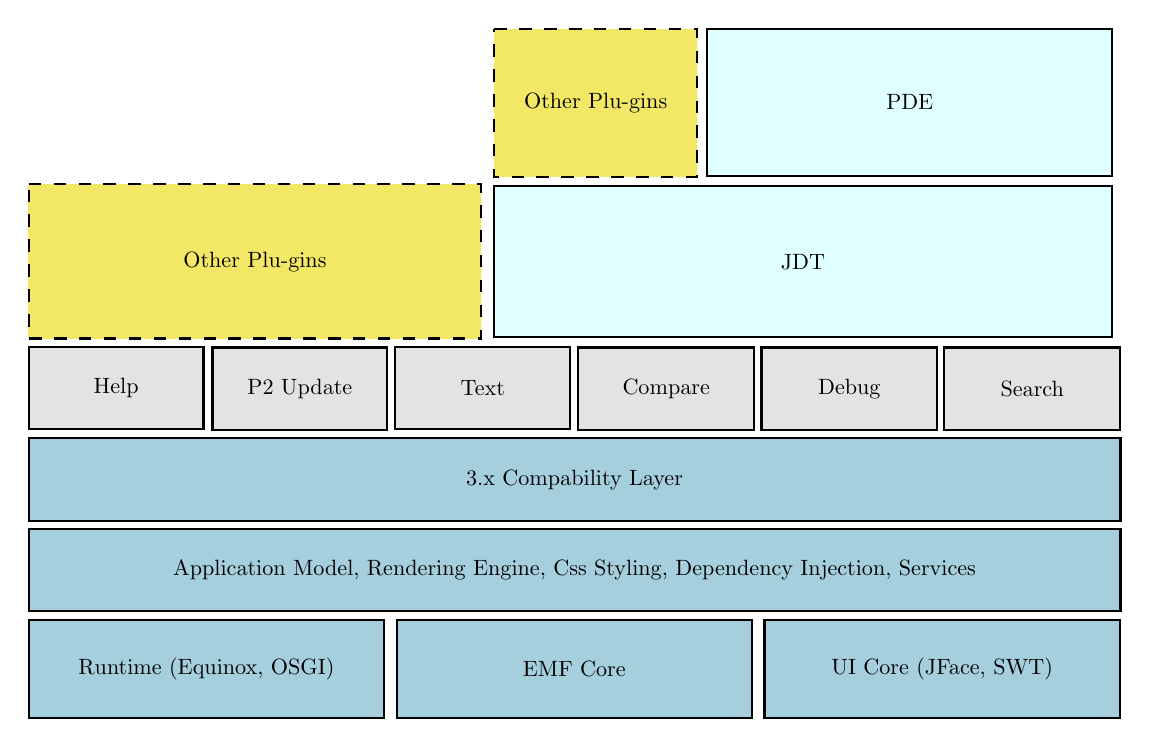
\begin{tikzpicture}[x=0.75pt,y=0.75pt,yscale=-1,xscale=1]
%uncomment if require: \path (0,451); %set diagram left start at 0, and has height of 451

%Shape: Rectangle [id:dp8432494375409605] 
\path  [shading=_wgbf5oer9,_zxnwhkf5u] (237.5,120) -- (535.5,120) -- (535.5,192.62) -- (237.5,192.62) -- cycle ; % for fading 
 \draw   (237.5,120) -- (535.5,120) -- (535.5,192.62) -- (237.5,192.62) -- cycle ; % for border 

%Shape: Rectangle [id:dp7026166067585526] 
\path  [shading=_8irm625ih,_1p7nvnkga] (13.5,328.84) -- (184.73,328.84) -- (184.73,376) -- (13.5,376) -- cycle ; % for fading 
 \draw   (13.5,328.84) -- (184.73,328.84) -- (184.73,376) -- (13.5,376) -- cycle ; % for border 

%Shape: Rectangle [id:dp6345226770671628] 
\path  [shading=_pjr06myd7,_gwc8z44gp] (367.99,328.84) -- (539.22,328.84) -- (539.22,376) -- (367.99,376) -- cycle ; % for fading 
 \draw   (367.99,328.84) -- (539.22,328.84) -- (539.22,376) -- (367.99,376) -- cycle ; % for border 

%Shape: Rectangle [id:dp5408347891690657] 
\path  [shading=_llx2ysmjf,_c0c5pm62p] (190.75,328.84) -- (361.98,328.84) -- (361.98,376) -- (190.75,376) -- cycle ; % for fading 
 \draw   (190.75,328.84) -- (361.98,328.84) -- (361.98,376) -- (190.75,376) -- cycle ; % for border 

%Shape: Rectangle [id:dp04645949367639268] 
\path  [shading=_pcsr14aqy,_rwos0a4s7] (13.5,285.04) -- (539.5,285.04) -- (539.5,324.67) -- (13.5,324.67) -- cycle ; % for fading 
 \draw   (13.5,285.04) -- (539.5,285.04) -- (539.5,324.67) -- (13.5,324.67) -- cycle ; % for border 

%Shape: Rectangle [id:dp28788690760284585] 
\path  [shading=_55iu8exu9,_8j056vhhr] (13.5,241.38) -- (539.5,241.38) -- (539.5,281) -- (13.5,281) -- cycle ; % for fading 
 \draw   (13.5,241.38) -- (539.5,241.38) -- (539.5,281) -- (13.5,281) -- cycle ; % for border 

%Shape: Rectangle [id:dp8477585057798736] 
\path  [shading=_i4lql9fyk,_nn1ckilfm] (13.5,119) -- (231.5,119) -- (231.5,193.25) -- (13.5,193.25) -- cycle ; % for fading 
 \draw  [dash pattern={on 4.5pt off 4.5pt}] (13.5,119) -- (231.5,119) -- (231.5,193.25) -- (13.5,193.25) -- cycle ; % for border 

%Shape: Rectangle [id:dp9553905279309911] 
\path  [shading=_8bwrpilif,_ofuilpt2d] (340.5,44) -- (535.5,44) -- (535.5,115) -- (340.5,115) -- cycle ; % for fading 
 \draw   (340.5,44) -- (535.5,44) -- (535.5,115) -- (340.5,115) -- cycle ; % for border 

%Shape: Rectangle [id:dp5609031712467787] 
\path  [shading=_dczef8aha,_cewc8yjbx] (278.29,197.6) -- (362.98,197.6) -- (362.98,237.22) -- (278.29,237.22) -- cycle ; % for fading 
 \draw   (278.29,197.6) -- (362.98,197.6) -- (362.98,237.22) -- (278.29,237.22) -- cycle ; % for border 

%Shape: Rectangle [id:dp8307768545013765] 
\path  [shading=_57ewcqsay,_dirmn7eue] (366.54,197.6) -- (451.23,197.6) -- (451.23,237.22) -- (366.54,237.22) -- cycle ; % for fading 
 \draw   (366.54,197.6) -- (451.23,197.6) -- (451.23,237.22) -- (366.54,237.22) -- cycle ; % for border 

%Shape: Rectangle [id:dp18083799783081855] 
\path  [shading=_yg605xfvy,_j8941ms5m] (454.68,197.6) -- (539.37,197.6) -- (539.37,237.22) -- (454.68,237.22) -- cycle ; % for fading 
 \draw   (454.68,197.6) -- (539.37,197.6) -- (539.37,237.22) -- (454.68,237.22) -- cycle ; % for border 

%Shape: Rectangle [id:dp6771550266372421] 
\path  [shading=_csrrlyr6m,_sn9stli8v] (190.16,197.4) -- (274.37,197.4) -- (274.37,237.02) -- (190.16,237.02) -- cycle ; % for fading 
 \draw   (190.16,197.4) -- (274.37,197.4) -- (274.37,237.02) -- (190.16,237.02) -- cycle ; % for border 

%Shape: Rectangle [id:dp09236116099021552] 
\path  [shading=_7h08hmb7r,_9vm1c694e] (102.03,197.6) -- (186.25,197.6) -- (186.25,237.22) -- (102.03,237.22) -- cycle ; % for fading 
 \draw   (102.03,197.6) -- (186.25,197.6) -- (186.25,237.22) -- (102.03,237.22) -- cycle ; % for border 

%Shape: Rectangle [id:dp05274071787404222] 
\path  [shading=_5afavzfur,_wvyo7vq6h] (13.5,197.2) -- (97.71,197.2) -- (97.71,236.82) -- (13.5,236.82) -- cycle ; % for fading 
 \draw   (13.5,197.2) -- (97.71,197.2) -- (97.71,236.82) -- (13.5,236.82) -- cycle ; % for border 

%Shape: Rectangle [id:dp3095230900303114] 
\path  [shading=_wptb90do4,_340xgp9yc] (237.83,44.29) -- (335.5,44.29) -- (335.5,115.25) -- (237.83,115.25) -- cycle ; % for fading 
 \draw  [dash pattern={on 4.5pt off 4.5pt}] (237.83,44.29) -- (335.5,44.29) -- (335.5,115.25) -- (237.83,115.25) -- cycle ; % for border 

% Text Node
\draw (122.5,156.31) node [scale=0.8] [align=left] {Other Plu-gins};
% Text Node
\draw (386.5,156.31) node [scale=0.8] [align=left] {JDT};
% Text Node
\draw (438,79.5) node [scale=0.8] [align=left] {PDE};
% Text Node
\draw (55.61,217.01) node [scale=0.8] [align=left] {Help};
% Text Node
\draw (144.14,217.41) node [scale=0.8] [align=left] {P2 Update};
% Text Node
\draw (232.27,217.21) node [scale=0.8] [align=left] {Text};
% Text Node
\draw (320.64,217.41) node [scale=0.8] [align=left] {Compare};
% Text Node
\draw (408.88,217.41) node [scale=0.8] [align=left] {Debug};
% Text Node
\draw (497.03,217.41) node [scale=0.8] [align=left] {Search};
% Text Node
\draw (276.5,261.19) node [scale=0.8] [align=left] {3.x Compability Layer};
% Text Node
\draw (276.5,304.86) node [scale=0.8] [align=left] {Application Model, Rendering Engine, Css Styling, Dependency Injection, Services};
% Text Node
\draw (99.11,352.42) node [scale=0.8] [align=left] {Runtime (Equinox, OSGI)};
% Text Node
\draw (276.36,352.42) node [scale=0.8] [align=left] {EMF Core};
% Text Node
\draw (453.61,352.42) node [scale=0.8] [align=left] {UI Core (JFace, SWT)};
% Text Node
\draw (286.67,79.95) node [scale=0.8] [align=left] {Other Plu-gins};


\end{tikzpicture}